% ============================================================================
% Networked Influence in a Tabula Rasa Legislature — Political Networks 2026
% Manchester. Slot: 25 min (18 talk + 7 Q&A). v1.
% Style: replicated from presentation-cpin2.tex / presentation-2026-07-23.tex.
% Compile: pdflatex presentation-polnet26.tex   (run twice: tikzmark overlays)
% ============================================================================
\documentclass[aspectratio=169,11pt]{beamer}

\usepackage[utf8]{inputenc}
\usepackage[T1]{fontenc}
\usepackage{amsmath, amssymb}
\usepackage{graphicx}
\usepackage{booktabs}
\usepackage{array}
\usepackage{xcolor}
\usepackage{qrcode}
\usepackage{tikz}
\usetikzlibrary{tikzmark, calc}

\usefonttheme{professionalfonts}
\usepackage{helvet}
\renewcommand{\familydefault}{\sfdefault}

\definecolor{ndred}{RGB}{222,32,38}
\definecolor{ndreddark}{RGB}{176,22,28}
\definecolor{ndgray}{RGB}{90,90,90}

\setbeamertemplate{navigation symbols}{}
\setbeamercolor{normal text}{fg=black,bg=white}
\setbeamercolor{structure}{fg=ndreddark}
\setbeamertemplate{itemize item}{\color{ndreddark}\textbullet}
\setbeamertemplate{itemize subitem}{\color{ndgray}\textendash}
\setbeamercolor{frametitle}{fg=black,bg=white}
\setbeamerfont{frametitle}{size=\large, series=\mdseries}
\setbeamertemplate{frametitle}{%
  \vspace{0.12cm}%
  \begin{center}\insertframetitle\end{center}%
  \vspace{-0.20cm}%
  {\color{ndred}\hrule height 1.1pt}}
\setbeamertemplate{footline}{%
  \hfill{\color{ndgray}\scriptsize\insertframenumber}\hspace{0.5cm}\vspace{0.2cm}}

\newcommand{\emphr}[1]{{\color{ndreddark}\textbf{#1}}}
\newcommand{\nota}[1]{{\footnotesize\color{ndgray} #1}}
\newcommand{\sectionslide}[2]{%
  \begin{frame}[plain]
    \vfill
    \begin{center}
      {\footnotesize\color{ndgray} #1}\\[6pt]
      {\Large #2}\\[2pt]
      {\color{ndred}\rule{0.30\textwidth}{1.1pt}}
    \end{center}
    \vfill
  \end{frame}}
% oval highlight: rounded rectangle between two tikzmark anchors
\newcommand{\ovalmark}[2]{\draw[ndred, very thick, rounded corners=7pt]
  ([shift={(-4pt,10pt)}]pic cs:#1) rectangle ([shift={(5pt,-4pt)}]pic cs:#2);}

% ---------------- Table A: profile homophily by bloc (macro, marks inside) ----
\newcommand{\TablaPerfil}{%
\begin{center}\tiny\setlength{\tabcolsep}{4pt}\renewcommand{\arraystretch}{1.12}
\begin{tabular}{lccccccc}
\toprule
\textbf{Same status}, by bloc of the pair & C1 & C2 & C3 & C4 & C5 & C6 & C7 \\
\midrule
\multicolumn{8}{l}{\emphr{--- Lawyer}}\\
\tikzmark{abogL}Left & $-0.07$ & $0.06$ & $0.02$ & $0.06^{+}$ & $0.00$ & $0.11^{*}$ & $-0.07$ \\
Center-left & $0.11$ & $0.11$ & $0.13$ & $-0.03$ & $0.15^{*}$ & $-0.26$ & $-0.00$ \\
Right & $-0.11$ & $-0.15^{**}$ & $-0.01$ & $0.01$ & $0.10$ & $0.13^{*}$ & $-0.06$ \\
Reserved seats & $0.06$ & $0.24$ & $0.10$ & $-0.26^{+}$ & $0.20^{*}$ & $-0.21$ & $-0.04$ \\
Others & $0.12$ & $-0.11$ & $-0.09$ & $0.09^{+}$ & $-0.00$ & $-0.13$ & $-0.15$ \\
Across blocs & $0.06$ & $-0.08^{*}$ & $0.02$ & $0.04^{*}$ & $-0.05^{+}$ & $0.07^{+}$ & $0.06^{+}$\tikzmark{abogR} \\
\multicolumn{8}{l}{\emphr{--- Prior institutional experience}}\\
\tikzmark{expL}Left & $0.12^{+}$ & $0.13^{*}$ & $0.09$ & $0.11^{**}$ & $0.04^{+}$ & $0.06$ & $0.00$\tikzmark{expR} \\
Center-left & $0.11$ & $-0.03$ & $0.09$ & $0.09^{**}$ & $-0.09$ & $-0.01$ & $0.12$ \\
Right & $-0.13$ & $-0.14$ & $-0.03$ & $0.05$ & $-0.14$ & $0.00$ & $-0.11$ \\
Reserved seats & $0.06$ & $0.00$ & $-0.08$ & $-0.05$ & $-0.11$ & $-0.10$ & $-0.05$ \\
Others & $-0.25$ & $-0.26$ & $--$ & $0.05$ & $--$ & $-0.20$ & $-0.30$ \\
Across blocs & $0.04$ & $0.06^{+}$ & $0.03$ & $0.06^{**}$ & $0.04^{*}$ & $0.04$ & $0.04$ \\
\multicolumn{8}{l}{\emphr{--- Gender}}\\
Left & $-0.12$ & $-0.03$ & $-0.06$ & $-0.03$ & $-0.02$ & $-0.04$ & $-0.09$ \\
Center-left & $-0.08$ & $-0.10$ & $-0.07$ & $0.00$ & $0.02$ & $-0.02$ & $0.05$ \\
Right & $0.14^{*}$ & $0.03$ & $0.05$ & $-0.06$ & $0.04$ & $-0.03$ & $0.09$ \\
Reserved seats & $-0.11$ & $-0.50$ & $-1.77$ & $-0.60^{**}$ & $-1.64^{***}$ & $0.04$ & $-0.26$ \\
Others & $-0.21$ & $-0.26$ & $-0.61$ & $-0.20^{**}$ & $-0.38^{*}$ & $0.19$ & $-0.37$ \\
\tikzmark{genL}Across blocs & $0.04$ & $0.12^{**}$ & $0.20^{*}$ & $0.13^{***}$ & $0.12^{***}$ & $0.08^{+}$ & $0.11^{*}$\tikzmark{genR} \\
\multicolumn{8}{l}{\emphr{--- District}}\\
\tikzmark{distL}Left & $-0.64^{*}$ & $-0.48^{*}$ & $0.45$ & $-0.45^{***}$ & $-0.29$ & $-0.45^{*}$ & $-0.04$ \\
Center-left & $-0.09$ & $-0.80$ & $-0.48$ & $0.73^{*}$ & $0.18$ & $-0.74$ & $0.30$ \\
Right & $1.00^{***}$ & $1.36^{***}$ & $0.42$ & $0.41^{***}$ & $0.08$ & $0.23$ & $0.88^{*}$ \\
Reserved seats & $-0.07$ & $0.13$ & $-0.03$ & $-0.27^{+}$ & $0.30$ & $-0.03$ & $0.19$ \\
Others & $1.98^{+}$ & $--$ & $-1.92^{**}$ & $--$ & $-0.29$ & $0.26$ & $--$ \\
Across blocs & $0.54^{***}$ & $0.28^{*}$ & $0.67^{**}$ & $0.39^{***}$ & $0.47^{***}$ & $0.34^{*}$ & $0.46^{**}$\tikzmark{distR} \\
\bottomrule
\end{tabular}
\end{center}}

% ---------------- Table B: controls + bloc spread + pre-network/structure -----
\newcommand{\TablaControles}{%
\begin{center}\tiny\setlength{\tabcolsep}{4pt}\renewcommand{\arraystretch}{1.3}
\begin{tabular}{lccccccc}
\toprule
 & C1 & C2 & C3 & C4 & C5 & C6 & C7 \\
\midrule
\multicolumn{8}{l}{\emphr{--- Controls}}\\
Edges (baseline) & $0.16$ & $-0.49$ & $-0.19$ & $-0.28$ & $-0.68$ & $-0.55$ & $-0.77$ \\
Commission member & $0.79^{***}$ & $1.60^{***}$ & $0.87^{***}$ & $1.06^{***}$ & $1.66^{***}$ & $1.96^{***}$ & $2.20^{***}$ \\
Range of $\theta_1$ per doc (global) & $-2.06^{***}$ & $-2.51^{***}$ & $-3.85^{**}$ & $-3.07^{***}$ & $-0.09$ & $-1.89^{*}$ & $-1.55$ \\
Range of $\theta_2$ per doc & $-2.10^{***}$ & $-1.49^{*}$ & $-1.73$ & $-2.35^{***}$ & $-2.02^{**}$ & $-1.49^{+}$ & $-0.71$ \\
\multicolumn{8}{l}{\emphr{--- Bloc internal spread ($\theta_1$ range of the own contingent, per doc)}}\\
\tikzmark{rngL}Left & $-1.21$ & $-1.16$ & $-2.75$ & $-3.70^{***}$ & $-3.81^{***}$ & $0.40$ & $-1.80$\tikzmark{rngR} \\
Center-left & $-1.76$ & $0.23$ & $0.23$ & $0.16$ & $-2.07$ & $3.35^{+}$ & $-1.54$ \\
Right & $0.20$ & $-0.30$ & $-5.29$ & $-5.33^{*}$ & $-6.92$ & $-0.45$ & $-3.03$ \\
Reserved seats & $-0.87$ & $0.94$ & $3.26$ & $-1.40$ & $-5.43^{+}$ & $0.15$ & $0.93$ \\
Others & $-4.82$ & $-2.71^{+}$ & $0.55$ & $-2.03^{**}$ & $-2.81^{***}$ & $-4.73^{*}$ & $-0.92$ \\
\multicolumn{8}{l}{\emphr{--- Pre-network variables and structure}}\\
Range of age per doc & $-0.26$ & $0.16$ & $-0.20$ & $0.03$ & $-0.57^{**}$ & $0.01$ & $0.17$ \\
Range of education per doc & $-0.27$ & $-0.57^{**}$ & $-0.28$ & $0.04$ & $-0.39^{*}$ & $-0.33$ & $-0.02$ \\
Serial signers (\texttt{gwb1degree}) & $-0.63$ & $-0.85$ & $-0.05$ & $-6.94^{*}$ & $-1.88^{***}$ & $1.22^{*}$ & $-0.55$ \\
\tikzmark{dspL}Repeated pairs (\texttt{gwdsp}) & $-0.42^{***}$ & $-0.28^{***}$ & $-0.38^{***}$ & $-0.16^{***}$ & $-0.23^{***}$ & $-0.35^{***}$ & $-0.24^{***}$\tikzmark{dspR} \\
\bottomrule
\end{tabular}
\end{center}}

% ============================================================================
\title{Networked Influence in a Tabula Rasa Legislature}
\author{Aníbal Olivera M. \& Jorge Fábrega L.}
\date{}

\begin{document}

% ------------------------------------------------------------------ 1 TITLE
\begin{frame}[plain]
  \vspace{0.6cm}
  \begin{center}
    {\footnotesize\color{ndgray} Political Networks 2026 $\cdot$ Manchester}
  \end{center}
  \vspace{0.9cm}
  \begin{center}
    {\LARGE \textbf{Networked Influence in a Tabula Rasa Legislature}}\\[0.45cm]
    {\large \color{ndreddark} Co-authorship, Ideological Dynamics, and Political Success\\in the Chilean Constitutional Convention (2021--2022)}
  \end{center}
  \vspace{1.0cm}
  \begin{center}
    {\normalsize Aníbal Olivera M. \quad$\cdot$\quad Jorge Fábrega L.}\\[2pt]
    {\footnotesize PhD(c) in Social Complexity Sciences, CICS--UDD, Chile}
  \end{center}
  \vfill
\end{frame}

% ------------------------------------------------------------------ 2 SETUP
\begin{frame}{A natural quasi-experiment}
\begin{itemize}
  \item In an ordinary legislature, today's collaboration network is the sediment of decades: careers, committees, party discipline.
  \vspace{0.25cm}
  \item The Chilean Constitutional Convention (Jul 2021 -- Jul 2022) started from \emphr{zero relational stock}: a majority of newcomers and independents, 17 reserved indigenous seats, a body that dissolved on delivery.
  \vspace{0.25cm}
  \item Each constitutional initiative required \emphr{8--16 sponsors}: signing = forming a visible coalition. 
  \vspace{0.25cm}
  \item Each norm needed \emphr{2/3 of the floor (103 of 154)}, so being born was cheap, but surviving was expensive.
\end{itemize}
\end{frame}

% ------------------------------------------------------------------ 3 DATA
\begin{frame}[plain]
\begin{center}
  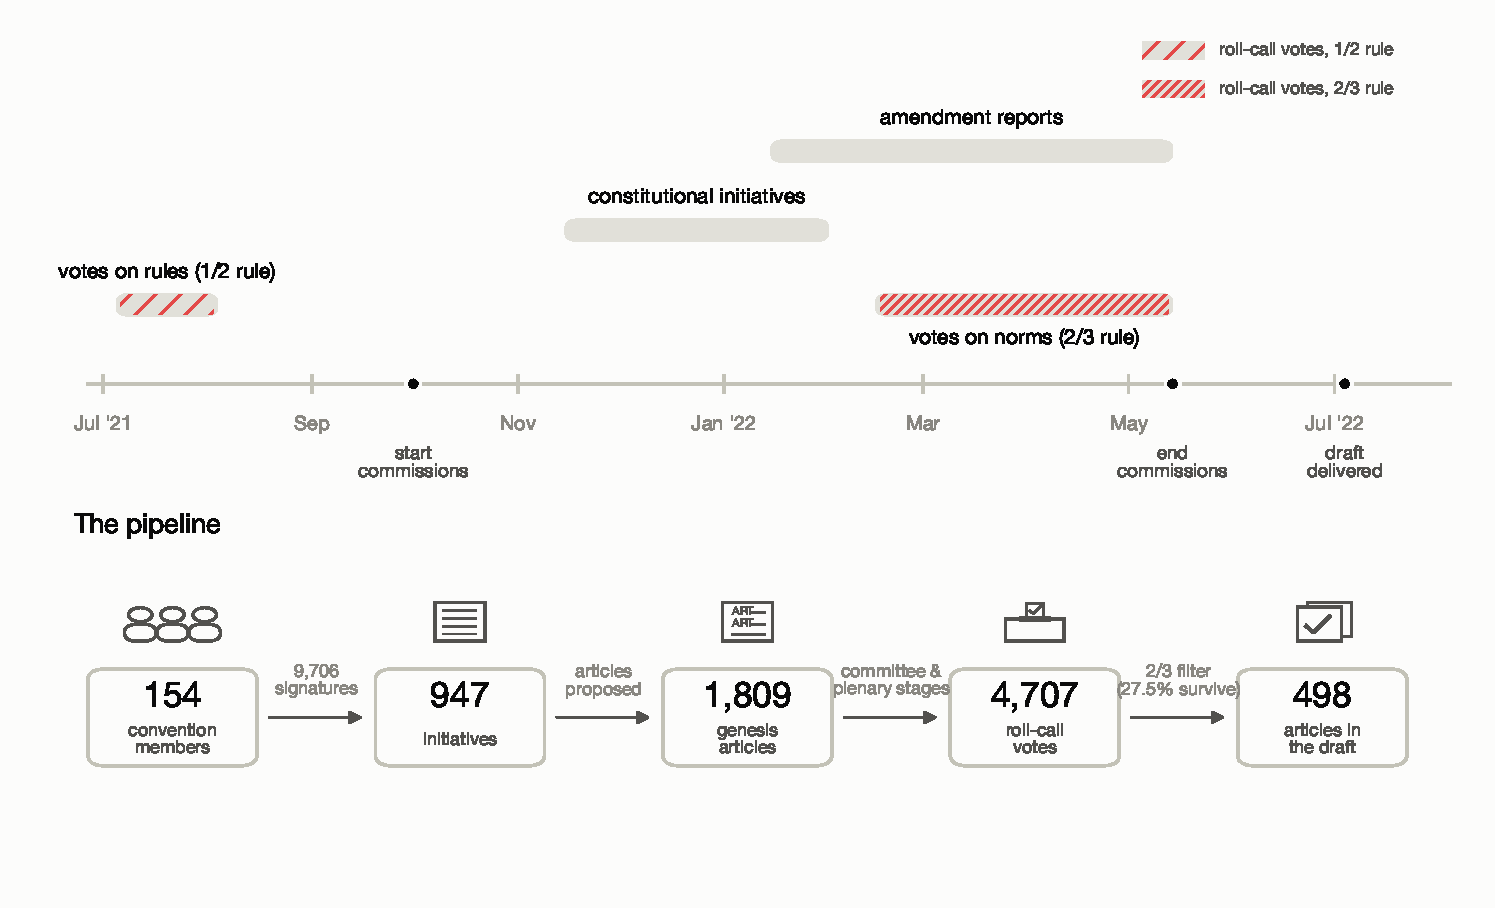
\includegraphics[width=0.97\textwidth]{../results/figures/data_infographic.pdf}
\end{center}
\end{frame}

% ------------------------------------------------------------------ 4 COMMISSIONS
\begin{frame}{What we know about each member}
\begin{itemize}
  \item \emphr{Political}: electoral list and bloc (Right / Center-left / Left / Reserved seats / Others); district of election.
  \vspace{0.2cm}
  \item \emphr{Profile}: age; gender; law degree; education level (HS / univ / master / PhD).
  \vspace{0.2cm}
  \item \emphr{Prior institutional experience}: had held elective or appointed public office before the Convention (former MPs, mayors, officials) — 35 of 154 members.
  \vspace{0.2cm}
  \item \emphr{Ideology}: two-dimensional ideal points from the first month of roll calls — measured \emph{before} the collaboration network existed.
\end{itemize}
\end{frame}

\begin{frame}{The seven thematic commissions}
\begin{center}\scriptsize\setlength{\tabcolsep}{3.5pt}
\begin{tabular}{clccccccc}
\toprule
 & Name (short) & Members & N lawyers & N exper. & Age & Education & Initiatives & Amd. Waves \\
\midrule
C1 & Political system & 25 & 15 & 9 & 42.2 & 1.44 & 89 & 4 \\
C2 & Const.\ principles & 18 & 4 & 4 & 45.8 & 1.28 & 114 & 3 \\
C3 & Form of the state & 30 & 11 & 12 & 45.1 & 1.43 & 51 & 6 \\
C4 & Fundamental rights & 30 & 9 & 4 & 45.9 & 1.03 & 283 & 5 \\
C5 & Environment & 19 & 4 & 3 & 44.7 & 1.26 & 133 & 5 \\
C6 & Justice systems & 17 & 15 & 3 & 42.6 & 1.65 & 93 & 6 \\
C7 & Knowledge systems & 15 & 2 & 0 & 51.7 & 1.33 & 64 & 8 \\
\bottomrule
\end{tabular}
\end{center}
\vspace{0.2cm}
\begin{itemize}
  \item Composition varies wildly across commissions — 15 of C6's 17 members are lawyers; C7 has no politically experienced member.
\end{itemize}
\end{frame}

% ------------------------------------------------------------------ 5 IDEOLOGY
\begin{frame}[plain]
\begin{center}
  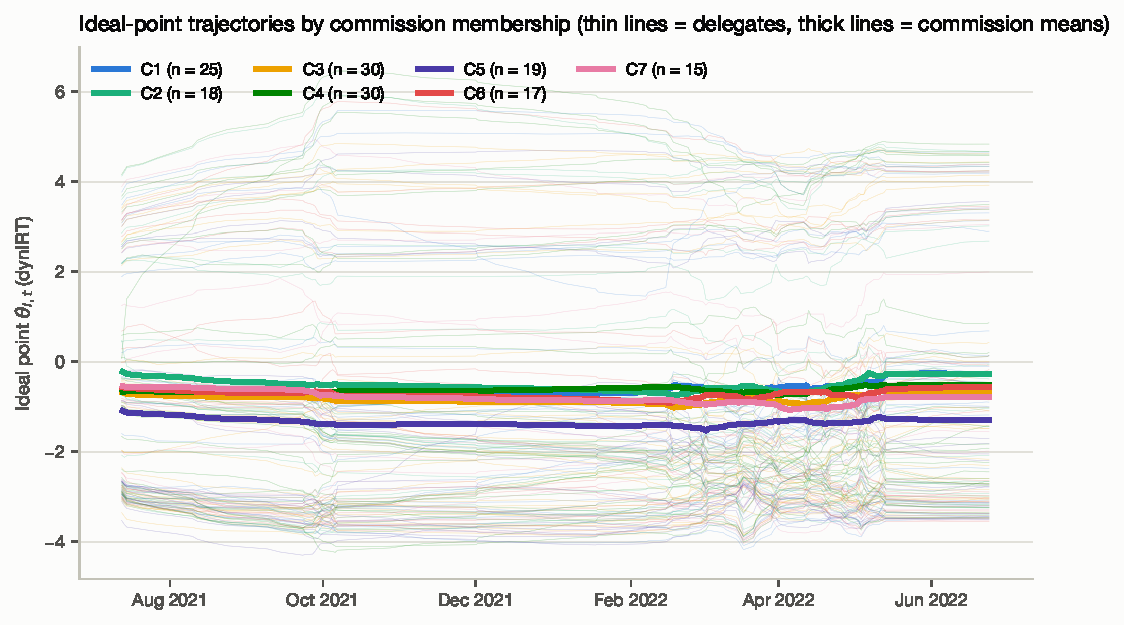
\includegraphics[width=1\textwidth]{../results/figures/positions_dynamics_by_commission.pdf}
\end{center}
\end{frame}

% ------------------------------------------------------------------ 6 RQs
\begin{frame}{Research questions}
\emphr{Formation}
\begin{itemize}
  \item \emphr{RQ1}: can the co-sponsorship network be predicted from what people \emph{brought with them} (district, lawyer, profile)?
\end{itemize}
\emphr{Behavior}
\begin{itemize}
  \item \emphr{RQ2a}: does network exposure \emph{move} members' ideological positions?
  \vspace{0.3cm}
  \item \emphr{RQ2b}: does voting \emph{defection} travel along co-sponsorship ties?
\end{itemize}
\emphr{Success}
\begin{itemize}
  \item \emphr{RQ3a}: what makes an \emph{article} survive into the draft?
  \vspace{0.3cm}
  \item \emphr{RQ3b}: does the \emph{context} an initiative is born into matter for its authors' success?
\end{itemize}
\end{frame}

\sectionslide{RQ1 — Formation}{Could we predict the network?}

% ------------------------------------------------------------------ 7 ERGM TOOL
\begin{frame}{Bipartite ERGM}
\begin{itemize}
  \item Unit of analysis: the \emphr{person - initiative} signature ($y_{ia} = 1$ if member $i$ signed initiative $a$).
\end{itemize}
{\small $$\Pr(Y = y) = \frac{\exp\big(\theta^\top s(y)\big)}{\kappa(\theta)}$$}
{\small $$
s(y) = \Big(\underbrace{\sum_{i,a} y_{ia}}_{\#\text{ edges}},\;\;
\underbrace{\sum_{a}\big(\max_{i:\,y_{ia}=1} v_i - \min_{i:\,y_{ia}=1} v_i\big)}_{\text{range of } v \text{ per doc}},\;\;
\texttt{gwb1deg},\;\; \texttt{gwdsp},\;\dots\Big)$$}
\begin{itemize}
  \item Variables: per-document ranges of $\theta_1, \theta_2$, age, education; the bloc contingent's own $\theta_1$ range; \texttt{gwb1degree}; \texttt{gwdsp}. 
  \item Seven models, one per commission.
  \item Estimation: MPLE as a logistic on change statistics; SEs by \emphr{initiative bootstrap} (B = 500).
\end{itemize}
\end{frame}

% ------------------------------------------------------------------ 8 TABLE A (4 overlays)
\begin{frame}[plain]
\TablaPerfil
\end{frame}

\begin{frame}[plain]
\TablaPerfil

\begin{tikzpicture}[remember picture, overlay]\ovalmark{abogL}{abogR}\end{tikzpicture}
\end{frame}

\begin{frame}[plain]
\TablaPerfil

\begin{tikzpicture}[remember picture, overlay]\ovalmark{expL}{expR}\end{tikzpicture}
\end{frame}

\begin{frame}[plain]
\TablaPerfil

\begin{tikzpicture}[remember picture, overlay]\ovalmark{genL}{genR}\end{tikzpicture}
\end{frame}

\begin{frame}[plain]
\TablaPerfil

\begin{tikzpicture}[remember picture, overlay]\ovalmark{distL}{distR}\end{tikzpicture}
\end{frame}

% ------------------------------------------------------------------ 9 TABLE B (2 overlays)
\begin{frame}[plain]
\TablaControles

\begin{tikzpicture}[remember picture, overlay]\ovalmark{rngL}{rngR}\end{tikzpicture}
\end{frame}

\begin{frame}[plain]
\TablaControles

\begin{tikzpicture}[remember picture, overlay]\ovalmark{dspL}{dspR}\end{tikzpicture}
\end{frame}

\sectionslide{RQ2 — People}{Does the network move positions (RQ2a) or behavior (RQ2b)?}

% ------------------------------------------------------------------ 10 RQ2a DESIGN
\begin{frame}{RQ2a design}
\begin{itemize}
  \item Only the \emphr{norms era} (Feb 15 -- May 14, content voted under the 2/3 rule).
  \item Exposure has \emphr{bounded memory}: network weights decay over time, parameterized by $m$ ($m=1 \approx 2$ weeks, $m=2 \approx 4$ weeks, $m=3 \approx 6$ weeks).
\end{itemize}
\vspace{0.3cm}
$$E^{(m)}_{i,t} = \frac{\sum_{j \neq i} w^{(m)}_{ij,t}\,\theta_{j,t}}{\sum_{j \neq i} w^{(m)}_{ij,t}},
\quad w^{(m)}_{ij,t} = \sum_{s \leq t} \lambda_m^{\,t-s} \Delta w_{ij,s}$$

$$
\Delta\theta_{i,t} = \alpha_i + \mu_t + \beta\,\theta_{i,t-1} + \lambda\,E^{(m)}_{i,t-1} + \lambda_{innov}\,\tilde E^{(m)}_{i,t+2} + \varepsilon_{it}$$
\begin{itemize}
  \item $\tilde E^{(m)}_{i,t+2}$: decay-weighted average of \emph{future} exposures.
\end{itemize}
\end{frame}

% ------------------------------------------------------------------ 11 F11


% ------------------------------------------------------------------ 12 DECAY
\begin{frame}{The result: the referee's test at three memories}
\begin{center}\small
\begin{tabular}{lccc}
\toprule
M2 (+ date FE + innovation $t{+}2$) & $m = 1$ ($\approx$ 2 wks) & $m = 2$ ($\approx$ 1 mo) & $m = 3$ ($\approx$ 6 wks) \\
\midrule
Lagged position $\theta_{i,t-1}$ ($\hat\beta$) & $-0.756^{***}$ & $-0.756^{***}$ & $-0.756^{***}$ \\
Decayed exposure $\hat\lambda$ ($E^{(m)}_{i,t-1}$) & $\mathbf{0.022^{***}}$ (0.006) & $\mathbf{0.022^{***}}$ (0.006) & $\mathbf{0.021^{***}}$ (0.006) \\
Decayed innovation $\hat\lambda_{innov}$ & $-0.008$ ($p=.25$) & $-0.007$ ($p=.38$) & $-0.005$ ($p=.60$) \\
Wave-date fixed effects & yes & yes & yes \\
N (person-waves) & 2,011 & 2,011 & 2,011 \\
$R^2$ within & 0.370 & 0.370 & 0.369 \\
\bottomrule
\end{tabular}
\end{center}
\vspace{0.25cm}
\begin{itemize}
  \item The lag stands at $\sim$0.022 — closing $\sim$2\% of the distance to the recent neighborhood per wave — and the \emphr{strictly future innovation predicts nothing}, at every memory.
  \item Honest label: an \emphr{influence component} that survives every test this panel supports; latent homophily cannot be excluded by design.
\end{itemize}
\end{frame}

% ------------------------------------------------------------------ 13 ERA 2/3


% ------------------------------------------------------------------ 14 RQ2b
\begin{frame}{RQ2b: defection — the design}
\begin{itemize}
  \item When someone breaks ranks: alone, or together with the people they wrote initiatives with?
\end{itemize}
\vspace{0.2cm}
$$X_{iv} = \frac{\sum_{j \neq i} w_{ij}\, D_{jv}}{\sum_{j \neq i} w_{ij}},
\qquad
\Pr(D_{iv} = 1) = \Lambda\big(\eta_i + \mu_{b(i),v} + \phi\, X_{iv} + \gamma\, marg_{iv}\big)$$
\begin{itemize}
  \item $\eta_i$ absorbs the born rebels; $\mu_{b(i),v}$ absorbs ``this vote split this bloc''.
  \item $\phi$ is the \emphr{parameter of interest}: do I defect more when my people defect?
  \item $marg_{iv}$: distance to one's own bloc's median position.
\end{itemize}
\end{frame}

\begin{frame}{RQ2b: the result (final model)}
\begin{center}\small
\begin{tabular}{lcc}
\toprule
 & Estimate & (SE) \\
\midrule
Exposure to defecting co-signers ($\phi$) & $\mathbf{8.75^{***}}$ & (0.61) \\
Marginality in own bloc ($\gamma$) & $1.09^{***}$ & (0.09) \\
\midrule
Fixed effects & \multicolumn{2}{c}{person + bloc $\times$ vote} \\
N (member-votes) & \multicolumn{2}{c}{186,988} \\
\bottomrule
\end{tabular}
\end{center}
\vspace{0.25cm}
\begin{itemize}
  \item Same bloc, same vote, same pressure: the members whose co-signers defect, \emphr{defect far more}.
  \item Marginality predicts defection strongly — the bloc's outsider breaks ranks — but takes \emph{nothing} from $\phi$: two independent channels.
  \item Carried by \emphr{newcomers at both ends} of the tie: novice receivers ($\phi = 12.2$ vs $9.5$) and novice senders alike.
\end{itemize}
\vspace{0.15cm}
\nota{Validation: shuffling \emph{who} defected within each bloc $\times$ vote (200 draws) puts the mechanics-only $\phi$ at 6.0; the raw two-way-FE number is 11.2. Full ladder in the paper.}
\end{frame}

\sectionslide{RQ3a — Texts}{What makes an article survive?}

% ------------------------------------------------------------------ 15 SURVIVAL
\begin{frame}{The survival model: article-level, complete}
\begin{itemize}
  \item We have 1,565 \emph{articles}, and 20.2\% of them reach the draft.
\end{itemize}
$$\Pr(\text{survives}_a) = \Lambda\Big(\alpha_c + \gamma_1\, \big|\bar\theta_{1,S_a} - \theta_{1,(103)}\big| + \gamma_2\, sd(\theta_{1,S_a}) + \gamma_3\, |S_a| + \boldsymbol{\gamma_4}^\top C_{S_a} + \boldsymbol{\gamma_5}^\top H_{S_a}\Big)$$
\begin{center}\scriptsize\setlength{\tabcolsep}{5pt}
\begin{tabular}{lccc}
\toprule
 & (1) Pivotal & (2) + Network & (3) + Human capital \\
\midrule
Coalition's distance to the $\tfrac{2}{3}$ pivot & $-0.35$ (\textbf{$p=.001$}) & $-0.48$ (\textbf{$p=.009$}) & $-0.61$ (\textbf{$p=.002$}) \\
Ideological heterogeneity $sd(\theta_1)$ & $+0.27$ (\textbf{$p=.008$}) & $+0.46$ (\textbf{$p=.001$}) & $+0.53$ (\textbf{$p<10^{-4}$}) \\
Coalition size & $+0.20$ ($p=.12$) & $+0.18$ ($p=.12$) & $+0.15$ ($p=.21$) \\
Mean betweenness & & $-0.22$ ($p=.083$) & $-0.23$ ($p=.076$) \\
Mean constraint & & $+0.01$ ($p=.97$) & $+0.26$ ($p=.28$) \\
Internal density (pairs with history) & & $+0.25$ (\textbf{$p=.024$}) & $+0.32$ (\textbf{$p=.002$}) \\
Share of lawyers & & & $-0.09$ ($p=.58$) \\
Share with prior experience & & & $-0.16$ ($p=.44$) \\
Mean academic degree & & & $-0.06$ ($p=.67$) \\
\midrule
AIC & 1393 & 1384 & 1386 \\
\bottomrule
\end{tabular}
\end{center}
\nota{Articles win by geometry (near the pivot, ideologically wide) and by teams with internal history — not by credentials.}
\end{frame}

% ------------------------------------------------------------------ 16 F12
\begin{frame}{Survival by coalition position: the arithmetic of 103}
\begin{center}
  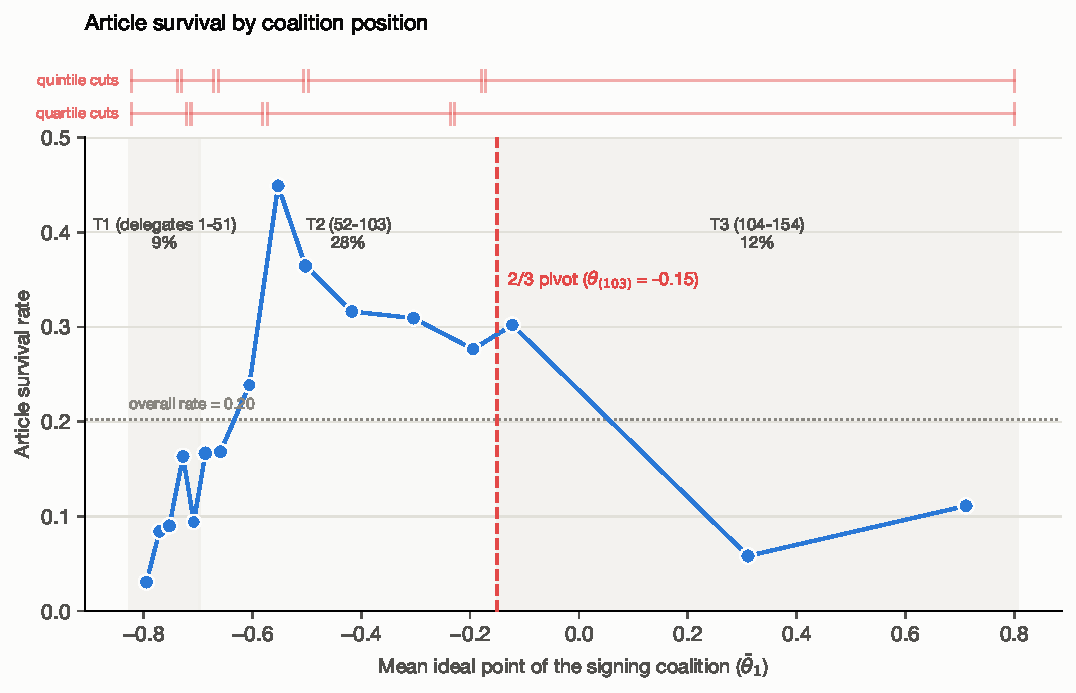
\includegraphics[width=0.78\textwidth]{../results/figures/survival_by_position.pdf}
\end{center}
\nota{The two-thirds rule fixed a pivot at $\theta_{1,(103)} = -0.15$. The premium for widening lives in left coalitions that can still reach the pivot by stretching; the sweet spot sits slightly left of the pivot — the center of mass of the drafting majority.}
\end{frame}

% ------------------------------------------------------------------ 17 SDM
\sectionslide{RQ3b — Members}{Whose success is it?}

\begin{frame}{Does the context an initiative is born into matter?}
\begin{itemize}
  \item \emphr{Success}: of all the article text you co-signed, how much survived into the draft? ($y_i$ = mean textual retention of $i$'s articles, 0 to 1.)
  \vspace{0.3cm}
  \item Success is \emphr{not individual}: it clusters on the co-sponsorship network (Moran's $I = 0.44$, $p \approx 10^{-163}$). Your success looks like your co-signers' success.
  \vspace{0.3cm}
  \item To test whether the company an initiative is born into matters, we relate each member's success to the \emph{average success of their co-signers}:
  $$y = \rho\, W y + X\beta + W X \gamma + \varepsilon,$$
  where $W$ is the row-normalized co-sponsorship network.
  \item One coefficient, $\rho$, answers whether that company matters.
\end{itemize}
\end{frame}

\begin{frame}{The full model}
\begin{center}\tiny\setlength{\tabcolsep}{4pt}\renewcommand{\arraystretch}{1.15}
\begin{tabular}{lcccc}
\toprule
 & Own ($\beta$) & $p$ & Co-signers' ($\gamma$, lag) & $p$ \\
\midrule
\multicolumn{5}{l}{\emphr{--- Activity and network position}}\\
Initiatives signed & $-0.0001$ & .28 & $+0.0002$ & .78 \\
Degree & $+0.0004$ & .30 & $+0.0052$ & .31 \\
Betweenness & $-0.0000$ & .98 & $-0.0020$ & .40 \\
\multicolumn{5}{l}{\emphr{--- Ideological position}}\\
Mean revealed vote ($\theta$) & $+0.008$ & .33 & $+0.056$ & .11 \\
SD of $\theta$ & $-0.018$ & .42 & $+0.026$ & .85 \\
Own distance to the $\tfrac{2}{3}$ pivot & $-0.002$ & .95 & $-0.265$ & \textbf{.050} \\
Ego heterophily & $-0.024$ & .088 & $-0.255$ & .055 \\
\multicolumn{5}{l}{\emphr{--- Credentials and profile}}\\
Lawyer & $+0.011$ & .13 & $+0.193$ & \textbf{.041} \\
Prior experience & $+0.019$ & \textbf{.031} & $+0.170$ & .11 \\
Academic degree & $-0.003$ & .49 & $-0.154$ & \textbf{.012} \\
Female & $+0.002$ & .78 & $+0.208$ & .075 \\
Age & $-0.0002$ & .53 & $-0.0033$ & .40 \\
\multicolumn{5}{l}{\emphr{--- Coupling}}\\
$\rho$ & $0.891$ & $\textbf{<.001}$ & — & — \\
\bottomrule
\end{tabular}
\end{center}
\end{frame}

\begin{frame}{Reading $\rho$: a spillover, up to identification}
\begin{itemize}
  \item The term $\rho\, W y$ is the \emph{equilibrium of an effort game}, and tell us the \emphr{coalition-effectiveness spillover}*: connected members' effectiveness spills over into yours (Battaglini et al., AJPS 2020).
  \vspace{0.3cm}
  \item And the covariates tell you what the ``context'' is made of: your own distance to the pivot doesn't matter ($p=.95$), your \emph{co-signers'} distance does ($-0.27$). \emphr{The context is the coalition you stand in.}
  \vspace{0.3cm}
  \item Taken together: the evidence supports the network view of success — where you stand shapes how well you do, beyond who you are.
\end{itemize}
\vspace{0.5cm}
\nota{* Up to an identification test currently in progress.}
\end{frame}

% ------------------------------------------------------------------ 18 TAKEAWAYS
\begin{frame}{Conclusions}
\begin{itemize}
  \item The network \emphr{was predictable} from what people brought with them: political bloc and — conditionally — shared district. Credentials organized nothing, in any bloc.
  \vspace{0.2cm}
  \item Territory is the right's internal glue and the system's bridge; gender crosses blocs; and \texttt{gwdsp} $< 0$ everywhere: coalitions re-form with fresh pairs — the \emphr{structural signature of a tabula rasa}.
  \vspace{0.2cm}
  \item In the norms era, positions \emphr{drift toward the recent neighborhood} ($\sim$2\% of the distance per wave), and the strictly-future placebo shows nothing: an influence component, not just selection.
  \vspace{0.2cm}
  \item Defection \emphr{travels along co-sponsorship ties} — same bloc, same vote, same pressure — carried by newcomers at both ends.
  \vspace{0.2cm}
  \item Articles win by \emphr{geometry and team history}, not credentials; and for the authors, \emphr{the context is the coalition}: success is a coalition good.
\end{itemize}
\end{frame}

% ------------------------------------------------------------------ 19 THANKS
\begin{frame}[plain]
  \vfill
  \begin{center}
    {\Large Thank you!}\\[2pt]
    {\color{ndred}\rule{0.22\textwidth}{1.1pt}}\\[0.8cm]
    \qrcode[height=2.6cm]{https://github.com/aoliveram/Networked-Influence-Chilean-Constitutional-Convention}\\[0.35cm]
    {\small GitHub project repository}\\[0.5cm]
    {\small\color{ndgray} anibal.olivera.m@gmail.com $\cdot$ aoliveram.cl}
  \end{center}
  \vfill
\end{frame}

\sectionslide{Backup}{Supporting material}

% ------------------------------------------------------------------ B1 MIXING
\begin{frame}{Backup: the bloc mixing matrix (pure closure, no profile counters)}
\begin{center}
  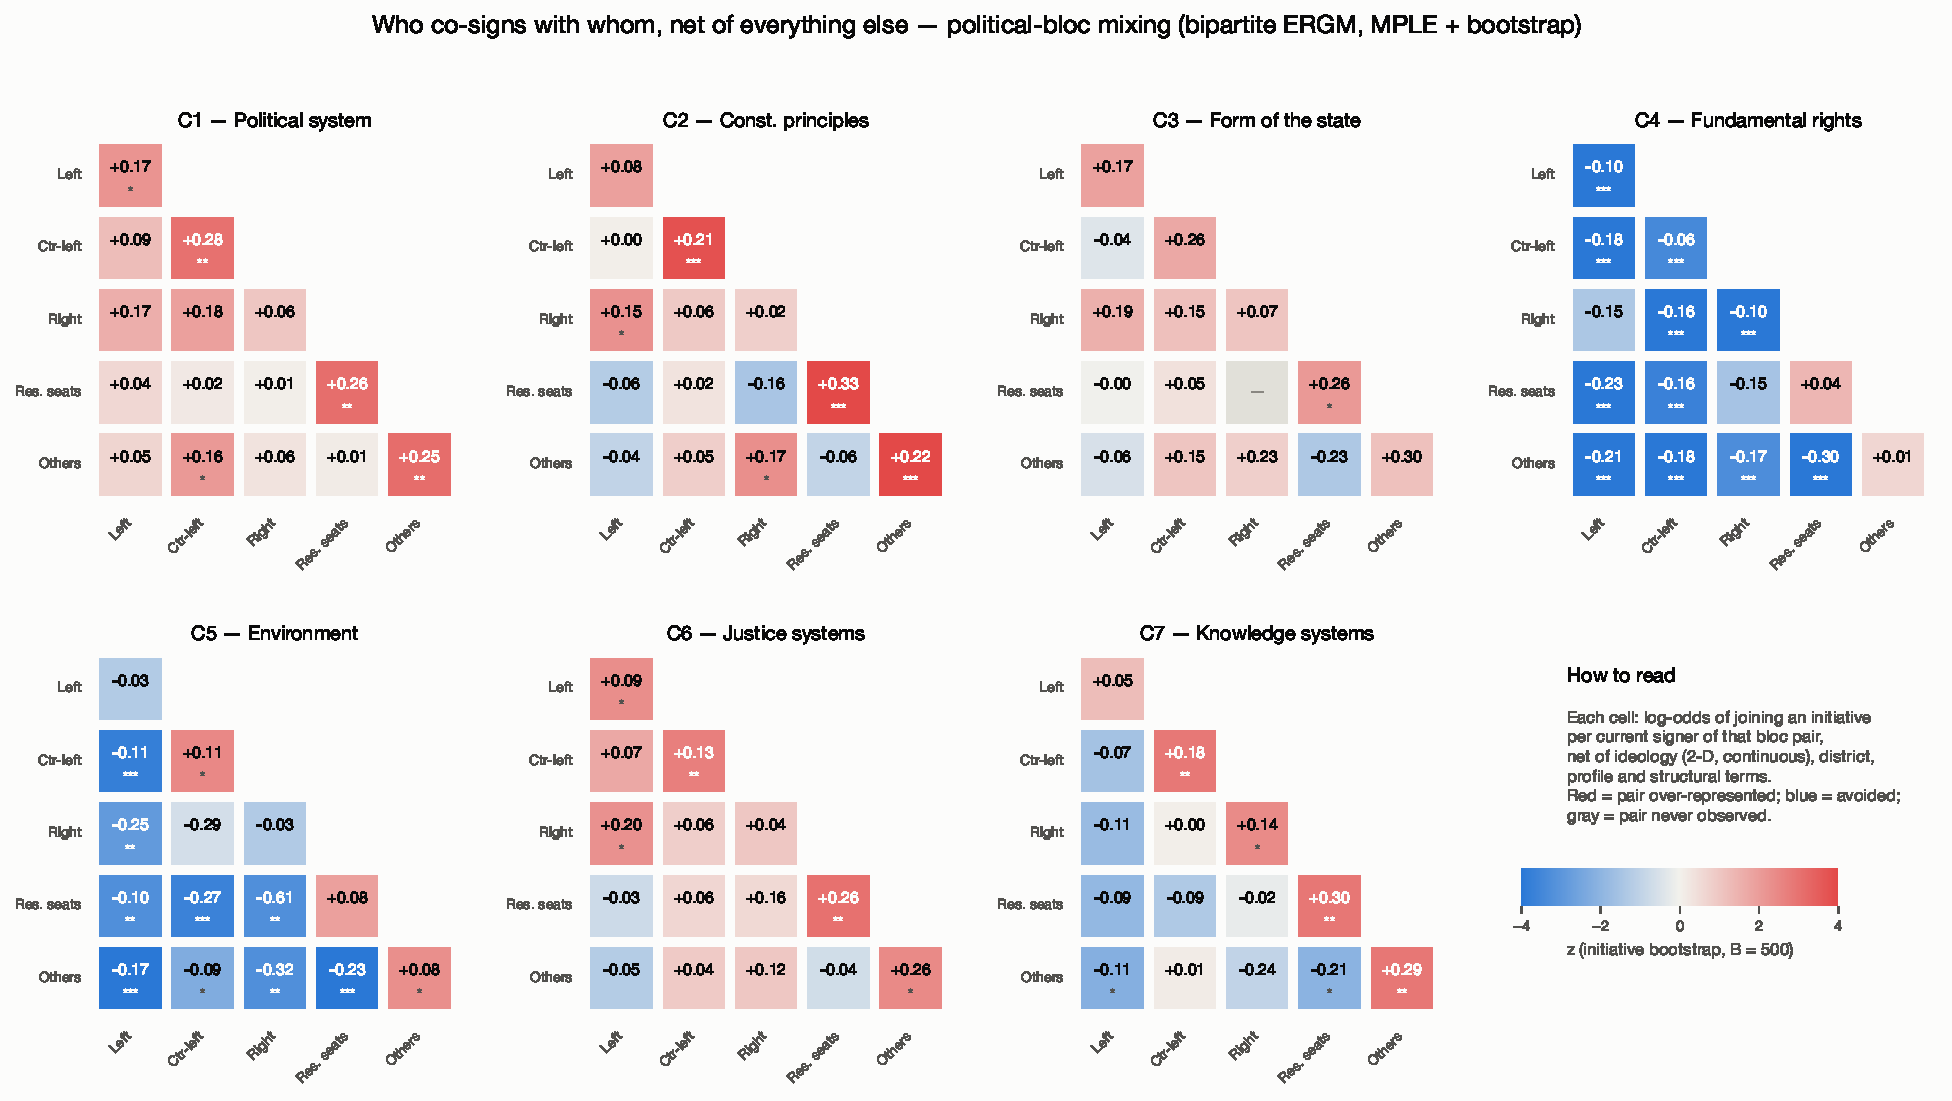
\includegraphics[width=0.9\textwidth]{../results/figures/nodemix_heatmap.pdf}
\end{center}
\end{frame}

% ------------------------------------------------------------------ B2 WINDOWS
\begin{frame}{Backup: the influence null, 3 windows $\times$ 7 exposure doses}
\begin{center}\tiny\setlength{\tabcolsep}{5pt}
\begin{tabular}{llcccc}
\toprule
Window & Exposure definition & $\hat\lambda$ & SE & $p$ & N \\
\midrule
Full & Accumulated since T0 & $+0.007$ & 0.004 & $0.119$ & 4,355 \\
Full & Last wave only & $+0.007$ & 0.013 & $0.60$ & 463 \\
Full & Last 2 waves & $+0.003$ & 0.009 & $0.72$ & 1,504 \\
Full & Last 3 waves & $-0.002$ & 0.007 & $0.76$ & 2,447 \\
Full & Decay $\lambda_w = 0.25 / 0.50 / 0.75$ & $+0.008/+0.008/+0.007$ & 0.004 & $.051/.042/.078$ & 4,355 \\
Full & Falsification: future exposure & $+0.010$ & 0.004 & $0.030$ & 3,329 \\
Early ($\leq$ Mar 31) & Accumulated & $+0.005$ & 0.007 & $0.50$ & 1,586 \\
Late ($\geq$ Apr 1) & Accumulated & $+0.011$ & 0.005 & $0.018$ & 2,769 \\
Late & Falsification: future exposure & $+0.010$ & 0.004 & $0.004$ & 1,742 \\
\bottomrule
\end{tabular}
\end{center}
\nota{No $\hat\lambda$ exceeds $0.011$; the few significant late-window lags come with an equally significant falsification of the same size.}
\end{frame}

% ------------------------------------------------------------------ B3 CLOGIT
\begin{frame}{Backup: how does each sector decide? (conditional logit, same data)}
\begin{center}\footnotesize
\begin{tabular}{lccccc}
\toprule
 & Right & Ctr-left & Left & Res.\ seats & Others \\
\midrule
Distance in $\theta_1$ & $-5.1^{***}$ & $-2.8^{**}$ & $-0.8$ & $+0.1$ & $-6.1^{***}$ \\
\bottomrule
\end{tabular}
\end{center}
\vspace{0.2cm}
\begin{itemize}
  \item The complementary lens: the conditional logit conditions within each initiative (menu) and can split by the \emph{decider's} bloc: the right almost never crosses ideological distance; the left crosses it all.
  \item The hybrid ERGM and the conditional logit agree on the substantive ranking — the tool changes what is visible, not what matters.
\end{itemize}
\end{frame}

\end{document}
